\documentclass[12pt,letterpaper]{article}
\usepackage{apa_manual}
\apatituloCorto{Datos en tiempo real y lectura de archivos}

\begin{document}

\apacabecera
  {Guía de datos en tiempo real: vintages, releases y lectura de archivos}
  {Manual teórico y práctico 1 — Organización e inspección de datos}
  {En este proyecto no queremos predecir usando la historia ya corregida que aparece hoy en las estadísticas oficiales, sino colocarnos exactamente en los zapatos del analista en cada mes histórico. Este documento explica qué archivos existen en el repositorio, qué significa cada columna y cómo cargarlos en Python sin contaminar las pruebas con información del futuro.}

\section{Por qué trabajamos con datos en tiempo real}

Cuando el Banco Central de Reserva del Perú (BCRP) publica por primera vez el crecimiento del PBI de un mes determinado, esa cifra inicial es preliminar. Conforme llegan más encuestas de empresas, estadísticas tributarias y cuentas trimestrales conciliadas, el BCRP corrige esa cifra en publicaciones posteriores \parencite{cruz2025}. Si tomáramos hoy la última tabla histórica de crecimiento del PBI y entrenáramos un modelo con ella, estaríamos cometiendo un error grave: asumir que en el año 2005 o en abril de 2020 ya se conocían revisiones que en realidad tardaron meses o años en calcularse \parencite{croushore2011}.

Para evitar esa trampa metodológica, la literatura macroeconómica distingue dos fechas diferentes para cada dato numérico:
\begin{enumerate}
  \item \textbf{Período objetivo ($t$ o \codigo{target\_period}):} el mes económico al que se refiere el crecimiento (por ejemplo, \codigo{2020m4} corresponde a abril de 2020).
  \item \textbf{Fecha de publicación o \emph{vintage} ($v$):} el mes en que apareció publicada la Nota Semanal o el informe oficial que contenía ese dato (por ejemplo, \codigo{2020m6} es junio de 2020, dos meses después).
\end{enumerate}

A partir de estos dos índices se define nuestra variable objetivo principal: la revisión acumulada a un horizonte fijo de \(H = 11\) meses posteriores a la primera estimación, expresada en puntos porcentuales (p.p.):
\begin{equation}
  Y_t^{(H)} = y_t^{(v_H)} - y_t^{(v_0)},
  \label{eq:revision_def}
\end{equation}
donde \(y_t^{(v_0)}\) es la primera cifra publicada para el mes \(t\) en su primer \emph{vintage} observable \(v_0(t)\), y \(y_t^{(v_H)}\) es la cifra que aparece para ese mismo mes \(t\) exactamente \(H\) meses después en \(v_H(t)\). Si \(Y_t^{(11)} > 0\), significa que la economía terminó revisándose al alza respecto al anuncio inicial.

\section{Anatomía del triángulo de revisiones y del formato releases}

La estructura bidimensional de publicaciones forma un \emph{triángulo de datos en tiempo real}, esquematizado en la Figura~\ref{fig:esquema_triangulo}. Cada fila representa una nueva edición mensual publicada (\emph{vintage}), mientras que cada columna corresponde a un mes económico evaluado. Al avanzar hacia abajo, los valores de una misma columna se van actualizando; la diagonal principal contiene las primeras publicaciones \(y_t^{(v_0)}\).

\begin{figure}[htbp]
  \caption{Esquema conceptual del triángulo de vintages y definición de la revisión \(Y_t^{(H)}\)}
  \label{fig:esquema_triangulo}
  \centering
  \begin{tikzpicture}[font=\small, >=Stealth]
    % Matriz ejemplo de 4x4
    \matrix (M) [matrix of nodes, draw=apaBorder, fill=apaBg, inner sep=4pt, ampersand replacement=\&,
      nodes={font=\small\normalfont, minimum width=1.75cm, minimum height=0.68cm, anchor=center}] {
      \textbf{\scriptsize Vintage \textbackslash\ Mes} \& \textbf{\scriptsize 2020m3} \& \textbf{\scriptsize 2020m4} \& \textbf{\scriptsize 2020m5} \\
      \texttt{2020m5} \& \(-16{,}3\) \& \(\cdot\) \& \(\cdot\) \\
      \texttt{2020m6} \& \(-16{,}7\) \& |[text=apaAccent, font=\small\bfseries]| \(-40{,}5\) \& \(\cdot\) \\
      \texttt{2020m7} \& \(-16{,}8\) \& \(-40{,}5\) \& \(-32{,}7\) \\
      \texttt{2021m5} \& \(-16{,}3\) \& |[text=apaNavy, font=\small\bfseries]| \(-39{,}1\) \& \(-32{,}8\) \\
    };
    \node[above=4pt of M-1-3, color=apaSlate] {\scriptsize Columna fija: mismo mes objetivo \(t\)};
    \node[right=10pt of M-3-4, align=left, font=\footnotesize] (n1) {Primera publicaci\'on \(y_t^{(v_0)}\)\\(\texttt{2020m4} visto en \texttt{2020m6})};
    \node[right=10pt of M-5-4, align=left, font=\footnotesize] (n2) {Publicaci\'on a \(H=11\) meses \(y_t^{(v_{11})}\)\\(\texttt{2020m4} visto en \texttt{2021m5})};
    \draw[->, color=apaAccent, thick] (M-3-3.east) to[out=12,in=180] (n1.west);
    \draw[->, color=apaNavy, thick] (M-5-3.south) to[out=-28,in=180] (n2.west);
    \node[below=8pt of M, align=center, font=\footnotesize, fill=white, draw=apaBorder, rounded corners=2pt, inner sep=4pt]
      {Revisi\'on observada en nuestro repositorio para \texttt{2020m4}: \(Y_{\text{2020m4}}^{(11)} = (-39{,}1) - (-40{,}5) = \mathbf{+1{,}4\text{ p.p.}}\)};
  \end{tikzpicture}
  \apanota{Valores reales de abril de 2020 en \codigo{output/analysis\_output/muestra\_objetivo\_gdp.csv} (el ejemplo ilustra la lógica diagonal del triángulo; los puntos indican meses aún no publicados en esa fecha).}
\end{figure}

Cuando se reorganiza el triángulo desplazando cada columna hacia arriba para alinear la primera estimación de todos los meses en una misma columna, se obtiene el formato \emph{releases}: allí las columnas se llaman \codigo{gdp\_1} (primera estimación), \codigo{gdp\_2} (segunda publicación), y así sucesivamente \parencite{cruz2025}. En este proyecto trabajamos con ambos enfoques, pero nuestro análisis econométrico y predictivo usa el horizonte fijo \(H=11\) meses sobre \emph{vintages} limpios, visualizados en la Figura~\ref{fig:triangulo_real}.

\begin{figure}[htbp]
  \caption{Mapa histórico completo del triángulo de vintages del PBI peruano (1994--2025)}
  \label{fig:triangulo_real}
  \centering
  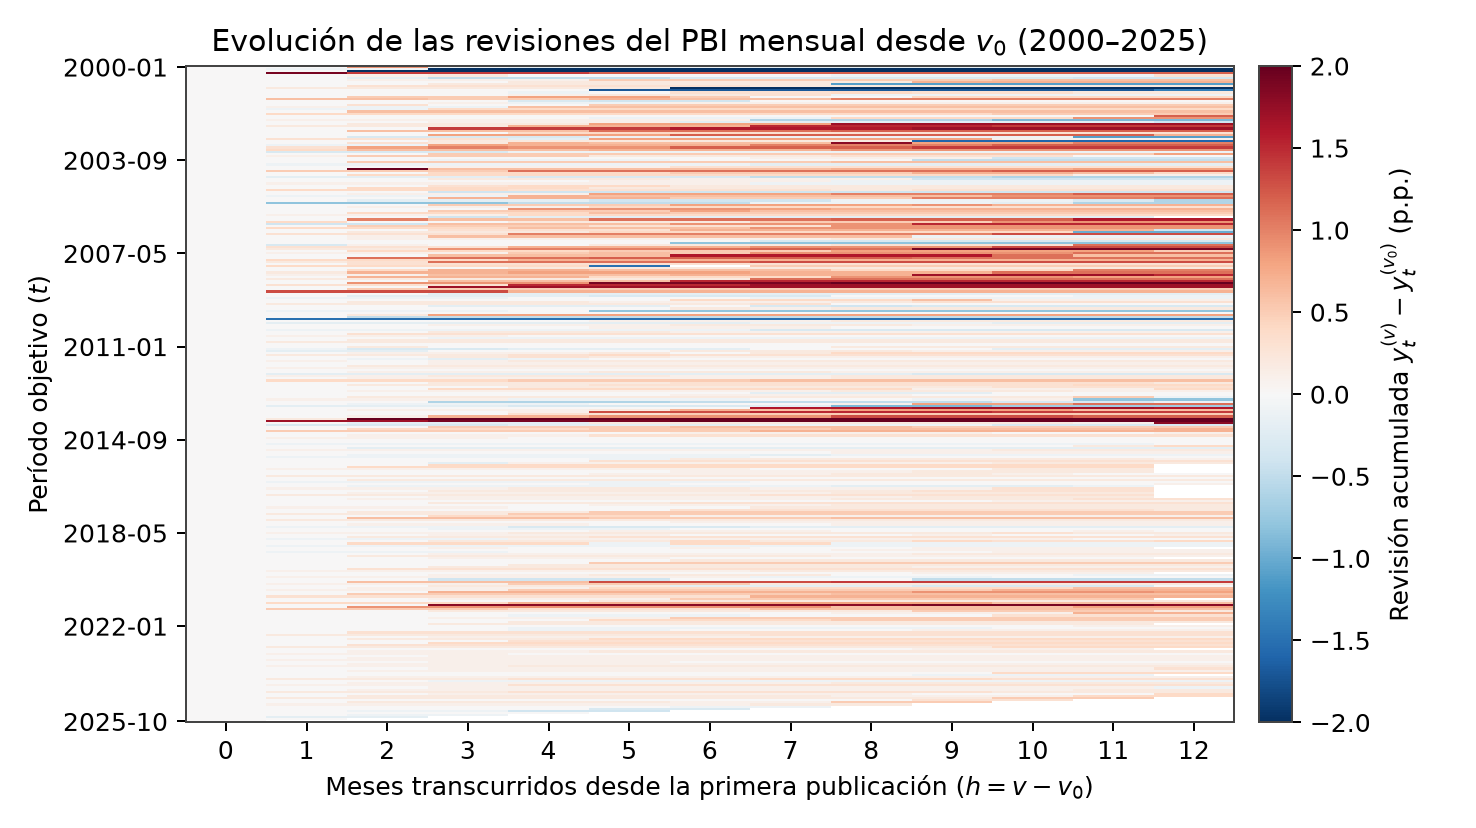
\includegraphics[width=0.92\textwidth]{figuras/triangulo_gdp.png}
  \apanota{Tomado de la auditoría de Etapa 1 (\codigo{output/analysis\_output/}). La diagonal inferior derecha representa el frente de publicaciones más recientes; cada salto vertical o franja continua refleja actualizaciones metodológicas o de año base.}
\end{figure}

\section{Mapa de carpetas y variantes del dataset}

Para trabajar con orden sin alterar nunca los datos originales, el proyecto separa claramente los insumos heredados de las salidas reproducibles generadas por nuestros scripts. La Tabla~\ref{tab:mapa_carpetas} resume qué contiene cada directorio relevante.

\begin{table}[htbp]
  \caption{Estructura práctica de carpetas de datos y resultados en el repositorio}
  \label{tab:mapa_carpetas}
  \centering
  \begin{tabular}{@{}p{4.3cm}p{4.4cm}p{5.8cm}@{}}
    \toprule
    Carpeta & Formato principal & Qué contiene y para qué sirve \\
    \midrule
    \codigo{raw/} & CSV con separador \codigo{;} & Tablas crudas históricas (1994--2012) extraídas y curadas desde Notas Semanales. \\
    \codigo{input/} & CSV y Parquet ancho & Tablas individuales estandarizadas por Nota Semanal (\codigo{table\_1}, \codigo{table\_2}). \\
    \codigo{peru\_gdp\_rtd\_output/} & CSV (\codigo{vintages/} y \codigo{releases/}) & Triángulo maestro consolidado en tiempo real (\(\approx 1994\text{--}2025\)) con sus variantes ajustadas. \\
    \codigo{output/analysis\_output/} & CSV, JSON, PNG & Auditoría de Etapa 1: serie larga \codigo{vintages\_long.csv} y muestra limpia \codigo{muestra\_objetivo\_gdp.csv}. \\
    \codigo{output/etapa2\_econometria/} & CSV, JSON, PNG & Pruebas estadísticas de sesgo, autocorrelación, Mincer--Zarnowitz y RESET. \\
    \codigo{output/etapa3\_clasicos/} & CSV, JSON, PNG & Predicciones causales OOS (2003m2--2024m11), métricas globales y por regímenes. \\
    \bottomrule
  \end{tabular}
  \apanota{Las tres primeras carpetas permanecen intactas como insumos base; las subcarpetas dentro de \codigo{output/} son regenerables íntegramente desde \codigo{scripts/}.}
\end{table}

Dentro de \codigo{peru\_gdp\_rtd\_output/output/vintages/} coexisten cuatro versiones del triángulo mensual. Es fundamental distinguirlas:
\begin{itemize}
  \item \codigo{monthly\_gdp\_vintages.csv}: cifras tal como fueron publicadas (incluye saltos bruscos cuando cambia el año base de las cuentas nacionales).
  \item \codigo{monthly\_gdp\_vintages\_adjusted.csv}: incorpora banderas o ajustes que identifican las transiciones de año base (en Perú ocurrieron en julio de 2000 y marzo de 2014).
  \item \codigo{...\_benchmark.csv} y \codigo{...\_adjusted\_benchmark.csv}: versiones filtradas para análisis de revisiones estándar sin rupturas metodológicas extremas.
\end{itemize}

\section{Cómo leer e interpretar los datos en Python}

En el trabajo diario rara vez necesitarás recorrer los 384 archivos de \codigo{input/} uno por uno. Según la tarea, conviene cargar directamente el triángulo maestro o la muestra ya auditada de la Etapa~1. El siguiente ejemplo práctico muestra cómo leer los cuatro tipos de archivos más frecuentes.

\begin{lstlisting}[language=Python, caption={Lectura práctica de datos crudos, vintages, releases y muestra limpia en Python}]
import pandas as pd

# 1. Leer una tabla historica cruda (separador ';' y BOM UTF-8)
raw_1994 = pd.read_csv(
    "raw/old_weekly_reports/table_1/1994/ns-03-1994.csv",
    sep=";", encoding="utf-8-sig"
)

# 2. Leer un archivo moderno de input en Parquet (2025)
inp_2025 = pd.read_parquet("input/table_1/2025/ns-04-2025.parquet")

# 3. Leer el triangulo maestro en formato ancho (408 columnas: tp_YYYYmM)
vintages = pd.read_csv(
    "peru_gdp_rtd_output/output/vintages/monthly_gdp_vintages.csv"
)
gdp_tri = vintages[vintages["industry"] == "gdp"].sort_values("vintage")

# 4. Leer la muestra limpia oficial lista para modelar (Etapa 1)
muestra = pd.read_csv(
    "output/analysis_output/muestra_objetivo_gdp.csv",
    parse_dates=["target_date", "v0_date", "v_H11_date"]
)
limpia_h11 = muestra[muestra["estado_H11"] == "incluido_limpio"]
print(limpia_h11[["target_period", "v0_date", "y0", "y_H11", "Y_H11"]].head())
\end{lstlisting}

Para interpretar correctamente \codigo{muestra\_objetivo\_gdp.csv}, recuerda tres reglas simples verificadas en la auditoría inicial:
\begin{enumerate}
  \item \textbf{Signo correcto:} la columna \codigo{Y\_H11} calcula \(y_t^{(v_{11})} - y_t^{(v_0)}\). En el repositorio existen columnas heredadas con el signo invertido (\codigo{first\_minus\_last}), por lo que siempre debe usarse \codigo{Y\_H11} o verificar que una media positiva indique revisión al alza.
  \item \textbf{Filtro \codigo{estado\_H11}:} los 24 períodos cuyo horizonte cruza un cambio de año base (`2000m7` o `2014m3`) y los meses sin primera publicación real en el momento oportuno (\codigo{lag0\_months > 3}) quedan marcados y excluidos al filtrar \codigo{incluido\_limpio}, dejando exactamente \(n=350\) observaciones continuas.
  \item \textbf{Sectores:} las seis ramas con cobertura completa o casi completa en tiempo real (\codigo{agriculture}, \codigo{commerce}, \codigo{construction}, \codigo{fishing}, \codigo{manufacturing} y \codigo{mining}) sirven como predictores, mientras \codigo{electricity} (desde 2003) y \codigo{services} (desde 1997) se reservan para análisis sectoriales parciales.
\end{enumerate}

\apabibliografia

\end{document}
